\section{Receptive Fields in the Retina and LGN}
\label{sec:ReceptiveFieldsInTheRetinaAndLGN}

\begin{defn}
  \label{def:ReceptiveFieldtype}
  A receptive field with a center-surround structure consisting either of a circular central ON region surrounded by an annular OFF region is called \emph{ON-center}, or the opposite arrangement of a central OFF region surrounded by an ON region is called \emph{OFF-center}.
\end{defn}

\begin{rem}
  Retinal ganglion cells display a wide variety of response characteristics, including nonlinear and direction-selective responses. However, a class of retinal ganglion cells (X cells in the cat or P cells in the monkey retina and LGN) can be described by a linear model built using reverse-correlation methods. The receptive fields of this class of retinal ganglion cells and an analogous type of LGN relay neurons are similar. The receptive fields of these neurons are ON-center or OFF-center.
\end{rem}

\begin{exm}
  \label{exm:ONcenterExm}
  The following figure shows the center-surround spatial structure of the receptive field of a cat LGN X cell. This has a central ON region (solid contours) and a surrounding OFF region (dashed contours).
  \begin{center}
    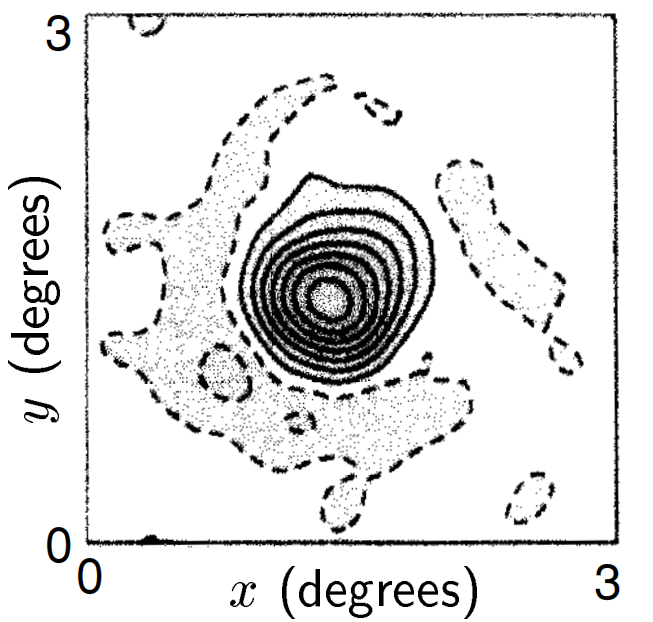
\includegraphics[scale=0.2]{./png/ONcenterExm}
  \end{center}
\end{exm}

\begin{defn}
  A \emph{difference-of-Gaussians model} capturing the spatial structure of retinal ganglion and LGN receptive fields is expressed as
  \begin{equation}
    \label{equ:2.45}
    D_s(x,y)=\pm\left(\frac{1}{2\pi\sigma_{\rm{cen}}^2}e^{-\frac{x^2+y^2}{2\sigma_{\rm{cen}}^2}}-\frac{B}{2\pi\sigma_{\rm{sur}}^2}e^{-\frac{x^2+y^2}{2\sigma_{\rm{sur}}^2}}\right),
  \end{equation}
  where the first Gaussian function describes the center, the second describes the surround, $\sigma_{\rm{cen}}$ determines the size of the central region, $\sigma_{\rm{sur}}$, which is greater than $\sigma_{\rm{cen}}$, determines the size of the surround, $B$ controls the balance between center and surround contributions, the $\pm$ sign allows both ON-center ($+$) and OFF-center ($-$) cases to be represented.
\end{defn}

\begin{exm}
  \label{exm:ONcenterEst}
  A fit of the receptive field shown in Example \ref{exm:ONcenterExm} using a difference-of-Gaussians function (Equation \ref{equ:2.45}) with $\sigma_{\rm{cen}} = 0.3^{\circ}$, $\sigma_{\rm{csur}} = 1.5^{\circ}$, and $B = 5$.
  \begin{center}
    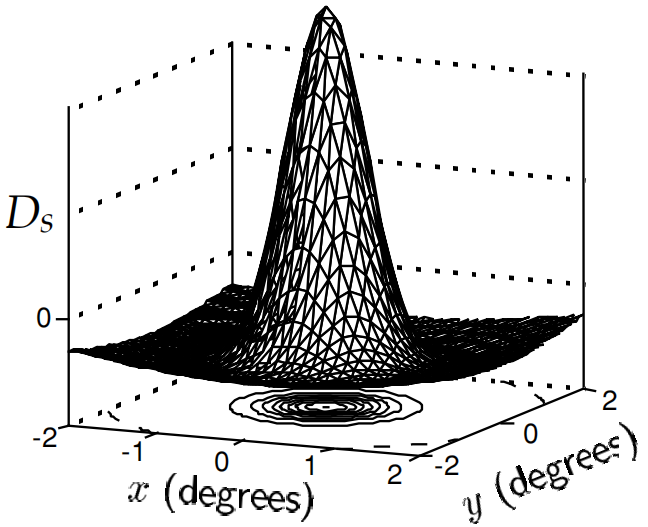
\includegraphics[scale=0.25]{./png/ONcenterEst}
  \end{center}
\end{exm}

\begin{exm}
  \label{exm:OFFcenterExm}
  The following figure shows the space-time receptive field of a cat LGN X cell.  Note that the center and surround regions both reverse sign as a function of $\tau$ and that the temporal evolution is slower for the surround than for the center.
  \begin{center}
    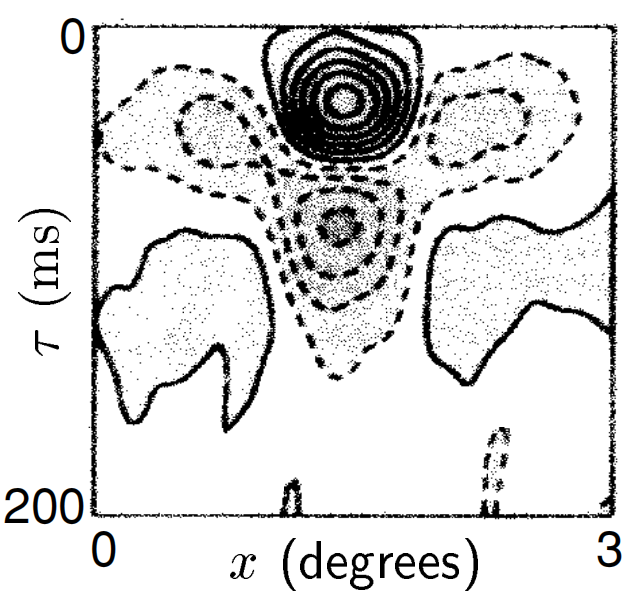
\includegraphics[scale=0.2]{./png/OFFcenterExm}
  \end{center}
  Because of the difference between the time course of the center and of the surround regions, the space-time receptive field is not separable, although the center and surround components are individually separable.
\end{exm}

\begin{defn}
  A model capturing basic features of LGN neuron space-time receptive fields is expressed as
  \begin{equation}
    \begin{aligned}
    \label{equ:2.46}
      D(x,y,\tau)=\pm\left(\frac{D_t^{\rm{cen}}(\tau)}{2\pi\sigma_{\rm{cen}}^2}e^{-\frac{x^2+y^2}{2\sigma_{\rm{cen}}^2}} - \frac{BD_t^{\rm{sur}}(\tau)}{2\pi\sigma_{\rm{sur}}^2}e^{-\frac{x^2+y^2}{2\sigma_{\rm{sur}}^2}}\right),
    \end{aligned}
  \end{equation}
  where $D_t^{\rm{cen}}(\tau)$ and $D_t^{\rm{sur}}(\tau)$ can both be described by the same functions, using two sets of parameters,
  \begin{equation}
    \label{equ:2.47}
    D_t^{\rm{cen},\rm{sur}}(\tau)=\alpha_{\rm{cen},\rm{sur}}^2\tau e^{-\alpha_{\rm{cen},\rm{sur}}\tau}-\beta_{\rm{cen},\rm{sur}}^2\tau e^{-\beta_{\rm{cen},\rm{sur}}\tau},
  \end{equation}
  where $\alpha_{\rm{cen}}$ and $\alpha_{\rm{sur}}$ control the latency of the response in the center and surround regions, respectively, and $\beta_{\rm{cen}}$ and $\beta_{\rm{sur}}$ affect the time of the reversal.
\end{defn}

\begin{rem}
   The function in Equation \ref{equ:2.47} has characteristics similar to the function in Equation \ref{equ:2.29}, but the latency effect is less pronounced.
\end{rem}

\begin{exm}
  \label{exm:OFFcenterEst}
   A fit of the space-time receptive field in Example \ref{exm:OFFcenterExm} using Equation \ref{equ:2.46} with the same parameters for the Gaussian functions as in Example \ref{exm:ONcenterEst}, and temporal factors given by Equation \ref{equ:2.47} with $1/\alpha_{\rm{cen}} = 16$ ms, $1/\alpha_{\rm{sur}} = 32$ ms, and $1/\beta_{\rm{cen}} = 1/\beta_{\rm{sur}} = 64$ ms.
  \begin{center}
    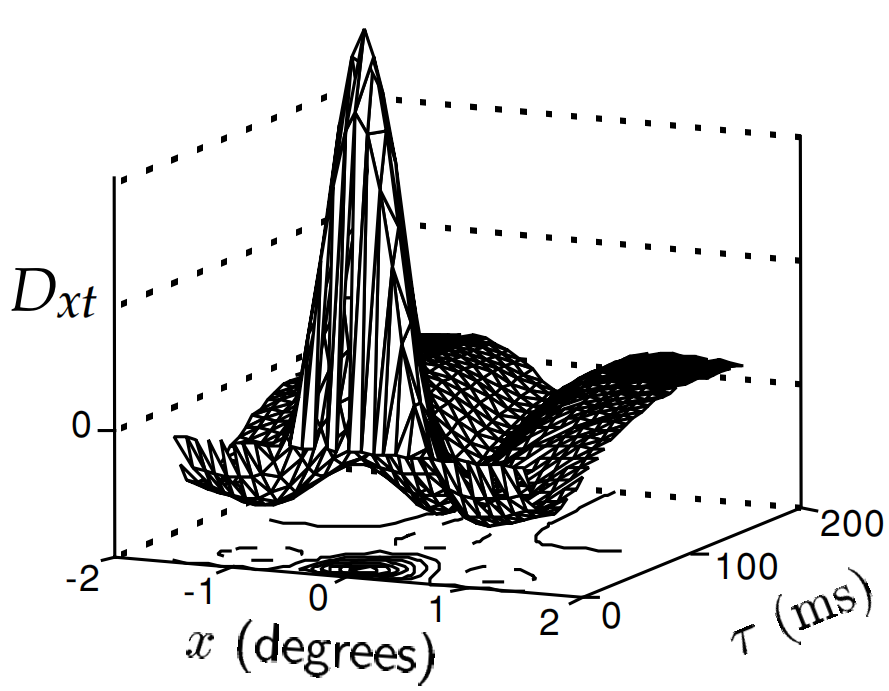
\includegraphics[scale=0.2]{./png/OFFcenterEst}
  \end{center}
\end{exm}

\begin{exm}[A direct test of a reverse-correlation model of an LGN neuron]
  \label{exm:directTestForLGN}
   Comparison of predicted and measured firing rates for a cat LGN neuron responding to a video movie is shown in the following figures.
  \begin{center}
    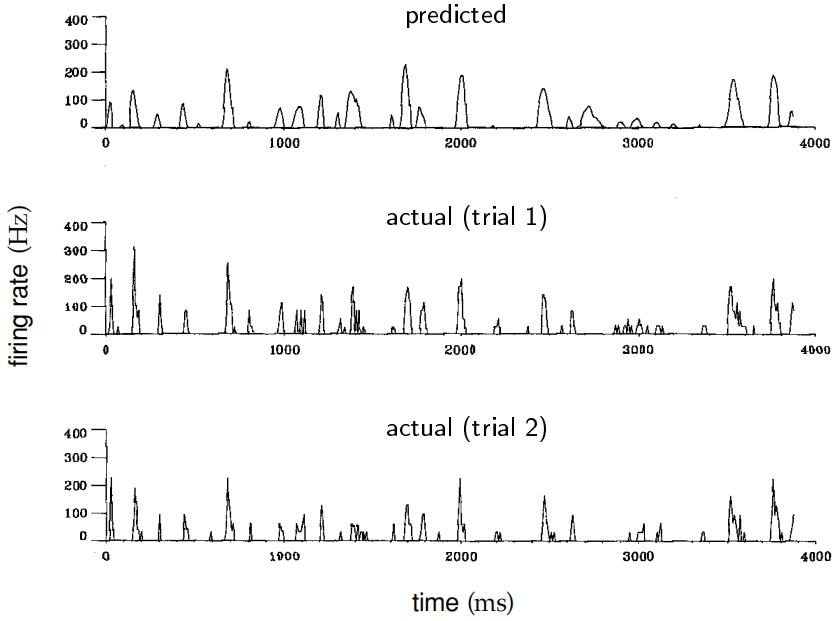
\includegraphics[scale=0.3]{./png/directTestForLGN}
  \end{center}
  \begin{enumerate}[(i)]
  \item The top panel is the rate predicted by integrating the product of the video image intensity and the kernel needed to describe this neuron was first extracted by using a white-noise stimulus. The resulting linear prediction was rectified, that is, $F(L) = G[L]_+$.
  \item The middle and lower panels are measured firing rates extracted from two different sets of trials.
  \end{enumerate}
\end{exm}

\begin{rem}
  In Example \ref{exm:directTestForLGN}, the correlation coefficient between the predicted and actual firing rates was 0.5, which was very close to the correlation coefficient between firing rates extracted from different groups of trials. This means that the error of the prediction was no worse than the variability of the neural response itself.
\end{rem}

%%% Local Variables:
%%% mode: latex
%%% TeX-master: "../notesOnFluidMechanics"
%%% End:
